\documentclass[11pt]{article}
\usepackage[a4paper,margin=24mm,headheight=15pt]{geometry}
\usepackage{fontspec}
\setmainfont{LiberationSerif-Regular.ttf}[Path=fonts/,BoldFont=LiberationSerif-Bold.ttf,ItalicFont=LiberationSerif-Italic.ttf,BoldItalicFont=LiberationSerif-BoldItalic.ttf]
\setsansfont{LiberationSans-Regular.ttf}[Path=fonts/,BoldFont=LiberationSans-Bold.ttf,ItalicFont=LiberationSans-Italic.ttf,BoldItalicFont=LiberationSans-BoldItalic.ttf]
\setmonofont{DejaVuSansMono.ttf}[Path=fonts/,Scale=0.83,BoldFont=DejaVuSansMono-Bold.ttf,ItalicFont=DejaVuSansMono-Oblique.ttf,BoldItalicFont=DejaVuSansMono-BoldOblique.ttf]
\usepackage{polyglossia}
\usepackage{amsmath,amssymb,booktabs,longtable,array,graphicx,xcolor}
\usepackage[font=small,labelfont=bf]{caption}
\usepackage{microtype}
\usepackage{placeins}
\usepackage{enumitem}
\setlist{nosep,leftmargin=*}
\usepackage[numbers,sort&compress]{natbib}
\usepackage[unicode,colorlinks=true,linkcolor=blue!45!black,citecolor=blue!45!black,urlcolor=blue!45!black]{hyperref}
\usepackage{xurl}
\usepackage{fancyhdr}
\pagestyle{fancy}\fancyhf{}\fancyhead[L]{\small\sffamily Spiking Bug}\fancyhead[R]{\small\sffamily Belkin · 2026}\fancyfoot[C]{\thepage}
\setlength{\parindent}{1.25em}\setlength{\parskip}{2pt}\setlength{\emergencystretch}{2em}
\linespread{1.06}
\graphicspath{{figures/}}
\newcommand{\code}[1]{\nolinkurl{#1}}
\newcommand{\CI}[3]{#1\,[#2,\,#3]}

\setdefaultlanguage{russian}\setotherlanguage{english}
\hypersetup{pdftitle={От прямых синапсов к нейромодуляции и ганглиям},pdfauthor={Андрей Белкин}}
\input{data/results-macros}
\title{От прямых синапсов к нейромодуляции и ганглиям:\\воспроизводимое исследование средств построения нервных схем и поведения агента в среде Spiking Bug}
\author{Андрей Белкин\\\small\href{mailto:it.belkin@gmail.com}{it.belkin@gmail.com}}
\date{21 октября 2026 г.}
\begin{document}
\maketitle
\begin{abstract}
Появление новых механизмов передачи сигналов и организации нервных систем может расширять множество схем, доступных эволюции, однако более богатое представление само по себе не гарантирует улучшения поведения. Представлена лаборатория Spiking Bug, объединяющая двумерную среду выживания, редактор коннектома, дискретные импульсные нейроны с утечкой, модулирующие синапсы и средства построения ганглиев. Исследуются три сохранённые схемы, по сообщению автора созданные агентом GPT-6 Astra по общему промпту с различиями в допустимых механизмах: сеть прямого действия D (17 нейронов), сеть с модуляцией M (19 нейронов) и ганглионарная сеть G (783 нейрона, включая 12 ганглиев). Использованы 60 общих случайных начальных сцен на условие и горизонт 1200 с; параметры схем в ходе оценки не изменялись. Среднее число собранных порций пищи составляет \DFood{}, \MFood{} и \GFood{}, а ограниченное среднее время жизни --- \DTime{}, \MTime{} и \GTime{} с. Однако отключение модуляции не изменяет зарегистрированные результаты M и повышает сбор пищи сетью G до \GNoModFood{} порций. Развёртывание ганглиев в явный граф сохраняет результаты трёх контрольных повторов. Таким образом, установлено различие эффективности конкретных схем, но не причинное преимущество модуляции или самой группировки нейронов. Разграничиваются динамические возможности, средства конструирования и эффективность использования ресурсов. Эволюционное развитие рассматривается как проверяемая инженерная аналогия, а не как реконструированная филогенетическая последовательность. К статье прилагаются исходные схемы, данные эпизодов, скрипты анализа, снимок кода среды и обе языковые версии рукописи.
\end{abstract}
\noindent\textbf{Ключевые слова:} спайковые нейронные сети; нейромодуляция; искусственная жизнь; ганглии; воплощённые агенты; эволюционные вычисления; воспроизводимость.

\section{Введение}
Нервная система связывает восприятие, внутреннее состояние организма и действие. Её совершенствование не обязательно сводится к увеличению числа нейронов: изменение доступных взаимодействий может менять способы интеграции сигналов, сохранения контекста и согласования конкурирующих моторных реакций. Отсюда возникает конструктивный вопрос: какие возможности появляются при переходе от прямых возбуждающих и тормозящих связей к модуляции, а затем к организованным популяциям нейронов?

Синтетический подход к изучению поведения имеет длительную историю. Модели Брайтенберга показывают, как сравнительно простые сенсомоторные связи могут порождать поведение, воспринимаемое как целенаправленное \citep{braitenberg1984}. Спайковые сети задают явный временной механизм взаимодействия возбуждения, торможения, задержек и рефрактерности \citep{gerstner2014}. В воплощённой модели результат возникает в замкнутом контуре: сеть меняет положение тела, положение меняет сенсорные сигналы, а они определяют дальнейшую активность сети. Поэтому анализ сети вне среды не заменяет испытания целостного агента.

Нейромодуляция представляет собой особый способ воздействия на этот контур. В биологических системах модуляторы способны изменять возбудимость и эффективные взаимодействия, позволяя одной анатомической сети формировать разные функциональные режимы \citep{marder2012}. Исследования небольших моторных цепей также показывают значение совместного действия ритмогенеза, сенсорной обратной связи и модуляторного управления \citep{marder2001}. Эти наблюдения мотивируют вычислительные механизмы, но не означают, что выбранная реализация воспроизводит конкретную нейромедиаторную систему. В данной работе модуляция --- ограниченное затухающее изменение чувствительности постсинаптического нейрона, без обучения сохранённых весов.

Популяционная организация решает другую задачу: упрощает описание, повторное использование и соединение больших групп клеток. В вычислительных моделях эволюции модульность может поддерживаться изменяющимися сочетаниями задач или стоимостью связей \citep{kashtan2005,clune2013}. Такие результаты относятся к определённым процессам отбора. Здесь сравниваются три фиксированные схемы, подготовленные для лаборатории. Поэтому оценивается их поведение в случайных сценах, а не вероятность обнаружения этих схем эволюцией и не скорость адаптации выбранного представления.

Работа решает три задачи. Во-первых, описывается исполнимая среда и инструментарий с явной семантикой, связывающей нейронные механизмы с наблюдаемым поведением. Во-вторых, проводится сравнение трёх сохранённых контроллеров по общему протоколу с отключением отдельных механизмов. В-третьих, устанавливаются границы аналогии между расширением средств построения схем и эволюцией нервных систем.

\begin{figure}[tbp]\centering
\includegraphics[width=\linewidth]{concept-ru.pdf}
\caption{Предлагаемая последовательность относится к средствам проектирования. Модуляция добавляет динамическое состояние чувствительности; ганглии предоставляют организацию популяций и сокращённое описание проекций. Стрелки не обозначают установленную историческую последовательность эволюции животных.}\label{fig:concept}
\end{figure}

\section{Биологические основания и границы аналогии}
Представление «прямая передача, затем модуляция, затем ганглии» удобно как порядок расширения возможностей лаборатории, но не должно трактоваться как универсальная биологическая лестница. Молекулярные компоненты, связанные с синапсами, имеют предшественников, возникших до появления нейронов \citep{ryan2009}. Гипотеза химического мозга допускает, что диффузная химическая коммуникация предшествовала синаптическим сетям \citep{jekely2021}; исследования ранних нейронных типов также подчёркивают роль секреторной специализации и разнообразия сигнальных систем \citep{burkhardt2021}. Поэтому программное добавление модуляции после прямых связей не задаёт времени её появления в природе.

История централизации нервных систем также не сводится к единственной линии. Согласно одному объяснению, нервные стволы и мозг возникают при расширении и интеграции более ранних нервных центров \citep{arendt2016}. Сравнительные данные развития поддерживают конвергентное происхождение ряда нервных стволов билатеральных животных \citep{martin2018}. Эти подходы побуждают исследовать организационные принципы, не утверждая, что одна последовательность описывает все эволюционные ветви.

Под \emph{эволюционной возможностью} здесь понимается механизм или форма описания, способные менять множество схем, доступных изменчивости и отбору. Необходимо различать три утверждения: механизм позволяет реализовать полезную динамику; конкретная схема получает от него преимущество; поиск с этим механизмом надёжнее находит эффективные схемы. Исследование фиксированных контроллеров проверяет второе утверждение в ограниченных условиях и характеризует первое на уровне реализации. Третье остаётся гипотезой для последующих эволюционных экспериментов.

\section{Материалы и методы}
\subsection{Архитектура лаборатории и происхождение схем}
Spiking Bug состоит из Python-сервера симуляции и двух клиентов на TypeScript/Vite. Клиент среды показывает агента, пищу, преследующие угрозы и физиологическое состояние. Редактор коннектома позволяет создавать нейроны, синапсы и ганглии, изменять параметры и наблюдать активность. Оба клиента используют единое состояние сервера. Переносимый JSON-документ содержит топологию, назначения сенсорных и моторных каналов, параметры мира и дополнительные метаданные. Проекции между ганглиями перед расчётом разворачиваются в индивидуальные связи.

Использована ревизия \code{befd6a0d53204722ade40be96000c3898b2158e5}. Входные схемы без настройки параметров скопированы из файлов \code{direct.json}, \code{modulation.json} и \code{ganglia-populatio.json}; последнее имя сохранено буквально. Копии и SHA-256 включены в материалы. Описания мира и назначения каналов во всех трёх файлах совпадают. D содержит 11 сенсорных, четыре моторных и два дополнительных нейрона; M --- четыре дополнительных нейрона; G --- 12 популяций по 64 нейрона и те же 15 сенсорных/моторных нейронов. Внутренний шум всех нейронов равен нулю.

По сообщению автора, схемы созданы агентом, обозначенным GPT-6 Astra. Общий промпт задавал цель выживания в течение 20 минут, начиная с дефолтных рецепторных и моторных нейронов. Агенту разрешалось создавать файл сохранения, проводить испытание, анализировать результат и дорабатывать схему до приемлемого поведения. Изменять код и настройки среды запрещалось; число нейронов и синапсов не ограничивалось. Между условиями различались разрешённые механизмы: прямое возбуждение/торможение, дополнительная модуляция и дополнительное использование ганглиев.

Автор предоставил точный промпт прямого варианта; общая основа и различия двух остальных вариантов сообщены автором, но не восстановлены по журналам генерации. Это итеративное конструирование с помощью LLM, а не однократная генерация и не биологический эволюционный процесс. Общая инструкция уменьшает различия в постановке задачи, однако не доказывает беспристрастность, равные затраты оптимизации или независимость эволюционных повторов. Точная версия модели, параметры генерации, количество обращений, кандидатов и испытаний, история отбора и seed оптимизации не предоставлены.

Сравниваемые файлы не образуют контролируемую последовательность добавления одного механизма. M отличается от D также прямыми связями и параметрами нейронов. G отличается размером, параметрами и топологией. Общие случайные сцены позволяют сопоставить целостные схемы, но не устраняют эти различия.

\begin{table}[tbp]\centering\small
\caption{Структура схем после развёртывания проекций. Знаки прямых связей определяются эффективными весами. Записи синапсов в файле могут описывать несколько индивидуальных связей.}\label{tab:structure}
\begin{tabular}{lrrr}\toprule
Характеристика & D & M & G\\\midrule
Нейроны &17&19&783\\
Ганглии &0&0&12\\
Записи синапсов &28&41&1887\\
Эффективные связи &28&41&3840\\
Положительные прямые связи &14&16&1856\\
Отрицательные прямые связи &14&23&1152\\
Связи модуляции возбуждения &0&2&640\\
Связи модуляции торможения &0&0&192\\\bottomrule
\end{tabular}
\end{table}

\begin{figure}[tbp]\centering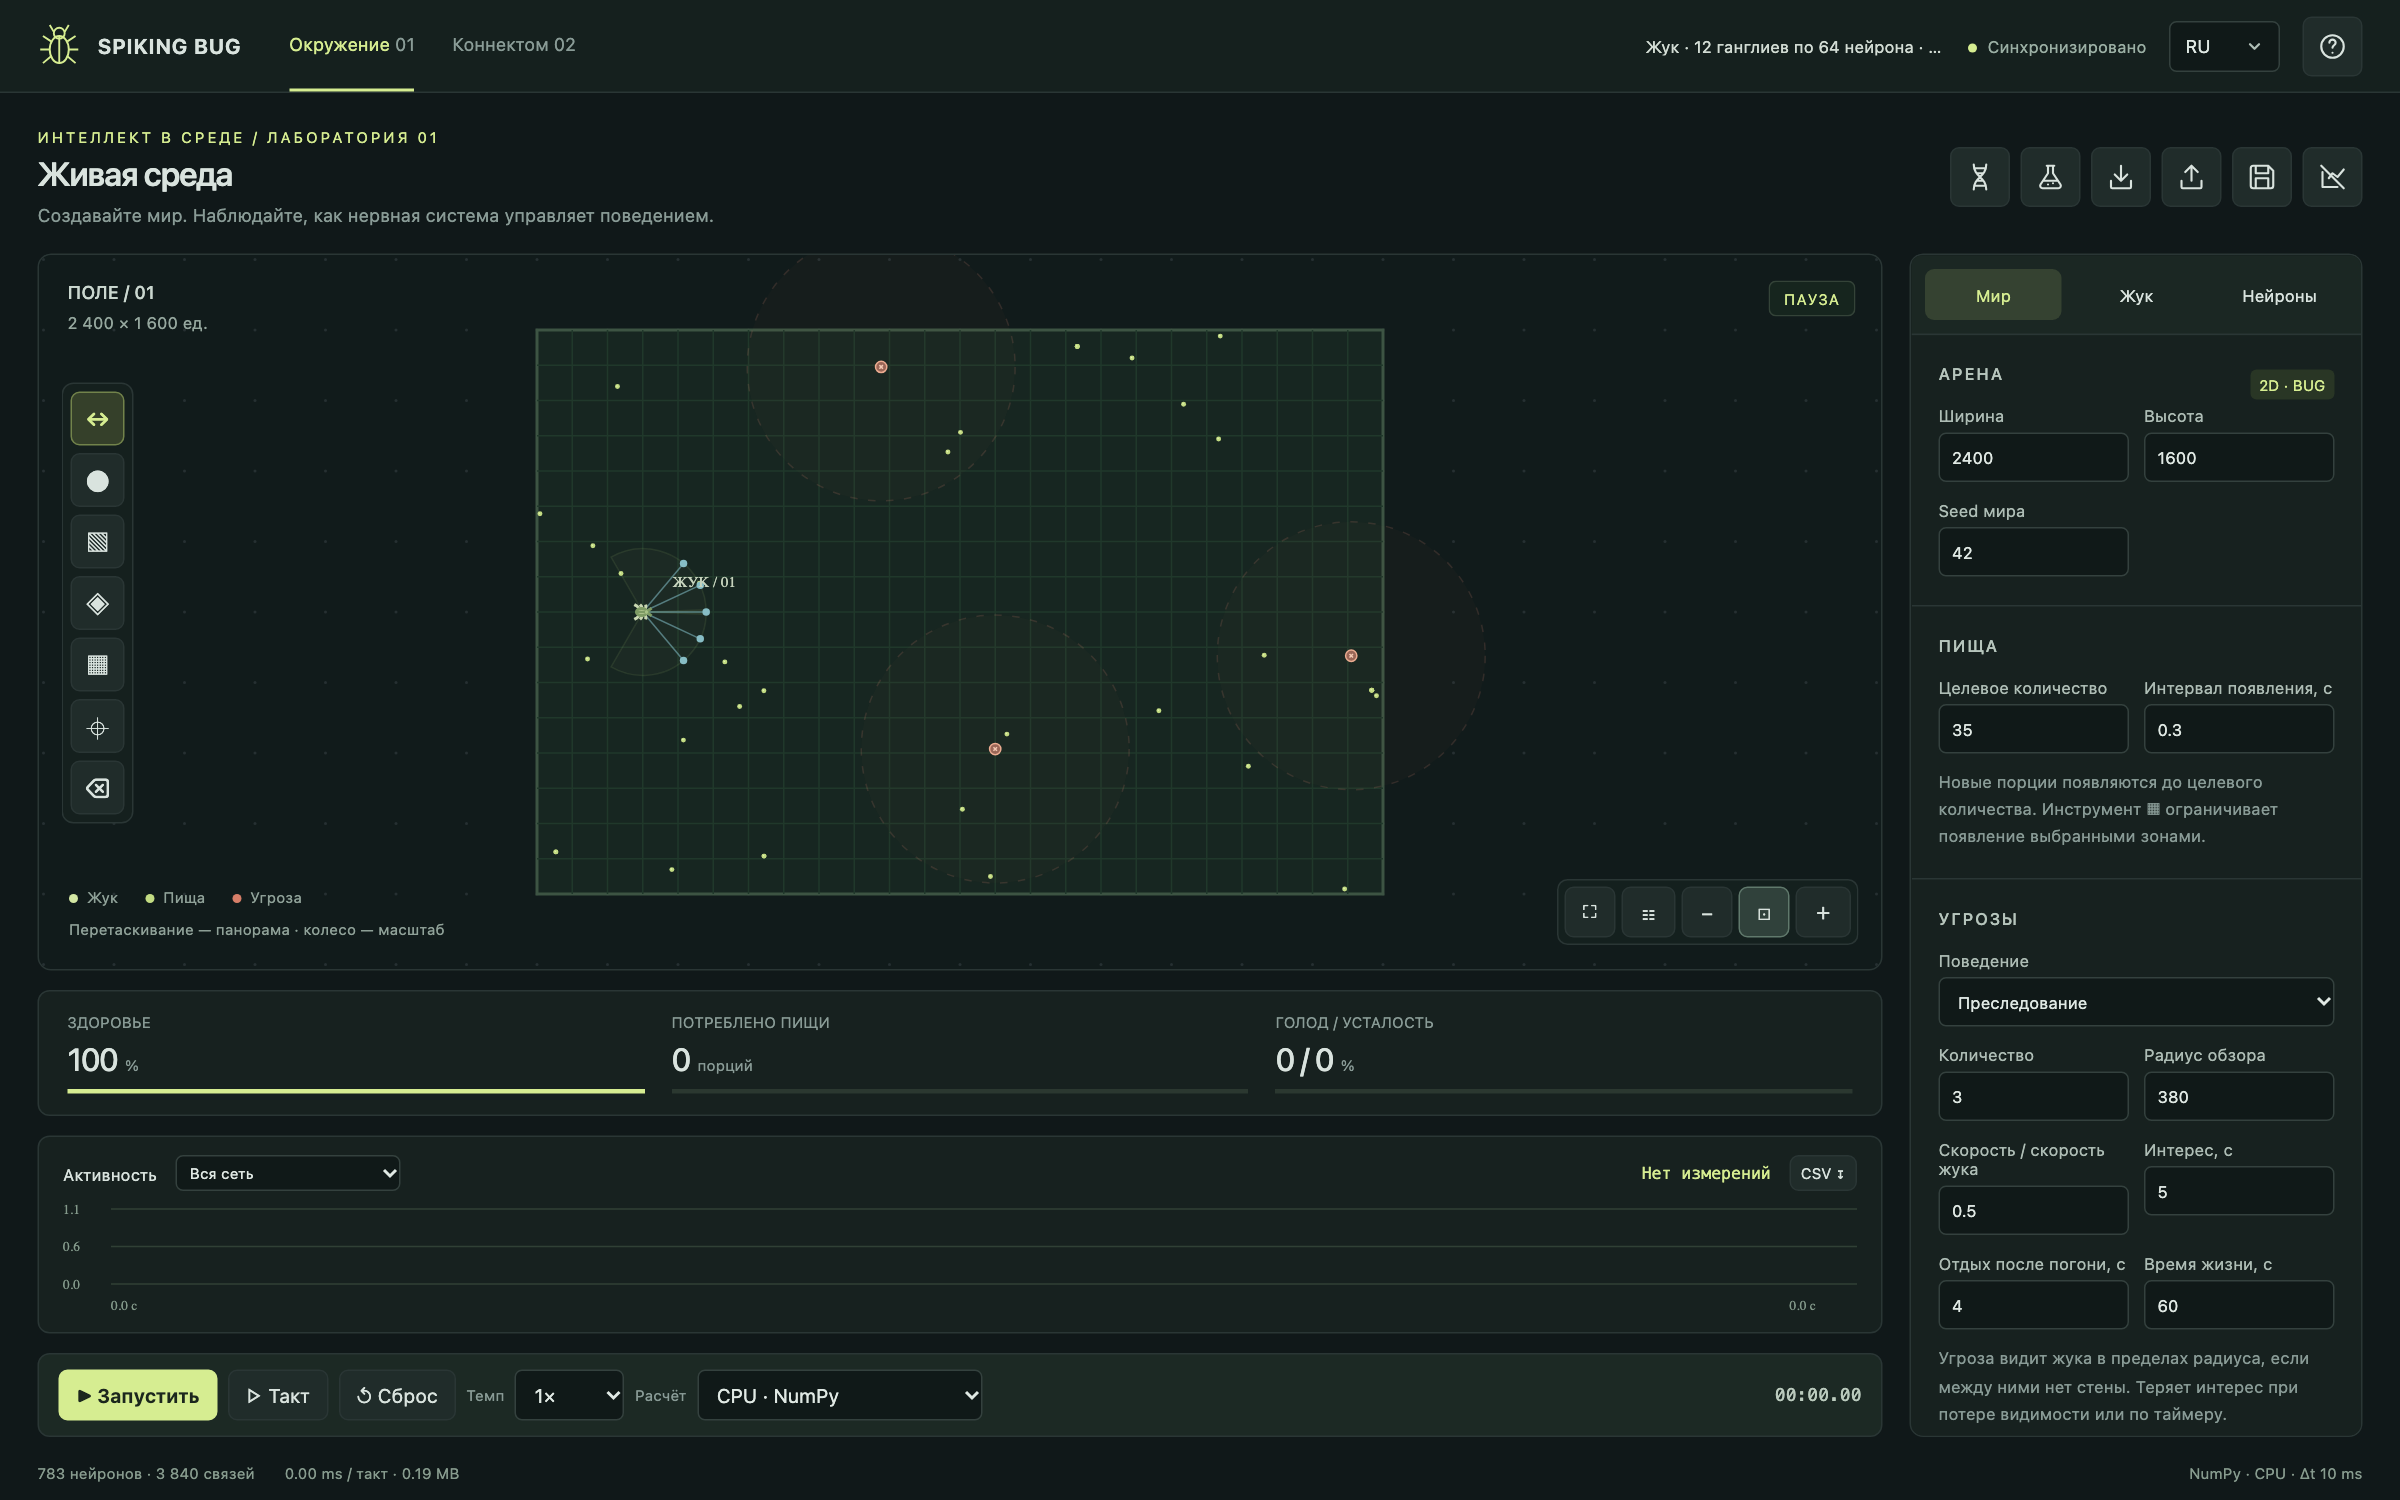
\includegraphics[width=\linewidth]{environment-ru.png}
\caption{Реальный интерфейс среды в изолированном локальном экземпляре с загруженной схемой G. Сохранённая сцена находится на паузе при $t=0$, seed 42. Снимок иллюстрирует среду и инструменты, а не специально выбранный успешный эпизод случайных испытаний.}\label{fig:environment}
\end{figure}

\subsection{Дискретная спайковая динамика}
Вычислитель CPU/NumPy использует шаг $\Delta t=0.01$ с. Пусть $V_i^t$ --- потенциал, $\lambda_i$ --- утечка за шаг, $b_i$ --- смещение и $u_i^t$ --- сенсорный вход. Прямые отложенные воздействия разделяются на положительную сумму $I_{i,+}^t$ и неположительную $I_{i,-}^t$. Две чувствительности $s_{i,+}$ и $s_{i,-}$ изменяются по правилу
\begin{equation}
\widetilde{s}_{i,q}^{t}=\operatorname{clip}_{[0,10]}\!\left[1+(s_{i,q}^{t-1}-1)e^{-\Delta t/\tau_{i,q}}+g_{i,q}M_{i,q}^{t}\right],\quad q\in\{+,-\},
\label{eq:mod}
\end{equation}
где $M_{i,q}^t$ --- сумма поступивших модулирующих весов, $g_{i,q}$ --- коэффициент усиления. Потенциал до пороговой проверки равен
\begin{equation}
\widetilde V_i^{t+1}=\operatorname{clip}_{[V_{i,\min},10^6]}\left[(1-\lambda_i)V_i^t+
\widetilde s_{i,+}^{t}I_{i,+}^t+\widetilde s_{i,-}^{t}I_{i,-}^t+b_i+u_i^t+\epsilon_i^t\right].
\label{eq:lif}
\end{equation}
Шум $\epsilon_i^t$ во всех исследованных схемах отсутствует. Спайк возникает при достижении порога, если в начале такта нейрон не был рефрактерным. Рефрактерность запрещает генерацию спайка, но не интеграцию потенциала. В режиме сброса реализация устанавливает потенциал в ноль; в режиме сохранения оставляет интегрированное значение. Поле \code{v_reset} не задаёт другое значение сброса в исследованном CPU-вычислителе. Утечка является дискретным коэффициентом, а не проводимостью в физических единицах.

Спайк помещает исходящие веса в кольцевой буфер задержек, измеренных целым числом тактов. Модуляция изменяет чувствительность к прямому синаптическому воздействию, но не к сенсорному входу или смещению, и не изменяет сохранённые веса. Поэтому механизм отличается от модулируемой синаптической пластичности, исследуемой в эволюционных обучающихся системах \citep{soltoggio2008}. Внутреннее состояние может сохранять недавний контекст без обучения весов, однако его польза зависит от схемы и задачи.

\subsection{Ганглии как форма представления}
Ганглий --- именованное множество конкретных нейронов и коннектор редактора. Проекция между группами размеров $n_a$ и $n_b$ разворачивается в $n_an_b$ индивидуальных связей. Каждый нейрон-источник передаёт собственные спайки: усреднения сигнала, отдельного состояния ганглия и дополнительной групповой задержки нет. Для прямой проекции из ганглия знак веса может определяться возбуждающей или тормозящей полярностью нейрона-источника. Поэтому структуру необходимо считать после развёртывания.

Если $\Phi$ --- оператор развёртывания, то динамика документа с ганглиями $G$ совпадает с динамикой графа $\Phi(G)$. Сама группировка не добавляет вычисления на уровне нейрона, а меняет способ задания схемы. При неограниченном бюджете добавление необязательных модулирующих связей включает прямые сети как частный случай с нулевой модуляцией: $\mathcal H_D\subseteq\mathcal H_M$. Ганглионарная запись, напротив, не доказывает строгого расширения класса явных графов при одинаковых механизмах и числе нейронов. Её возможное преимущество связано с организацией, повторным использованием и тем, какой поиск порождает такая запись.

\begin{figure}[tbp]\centering
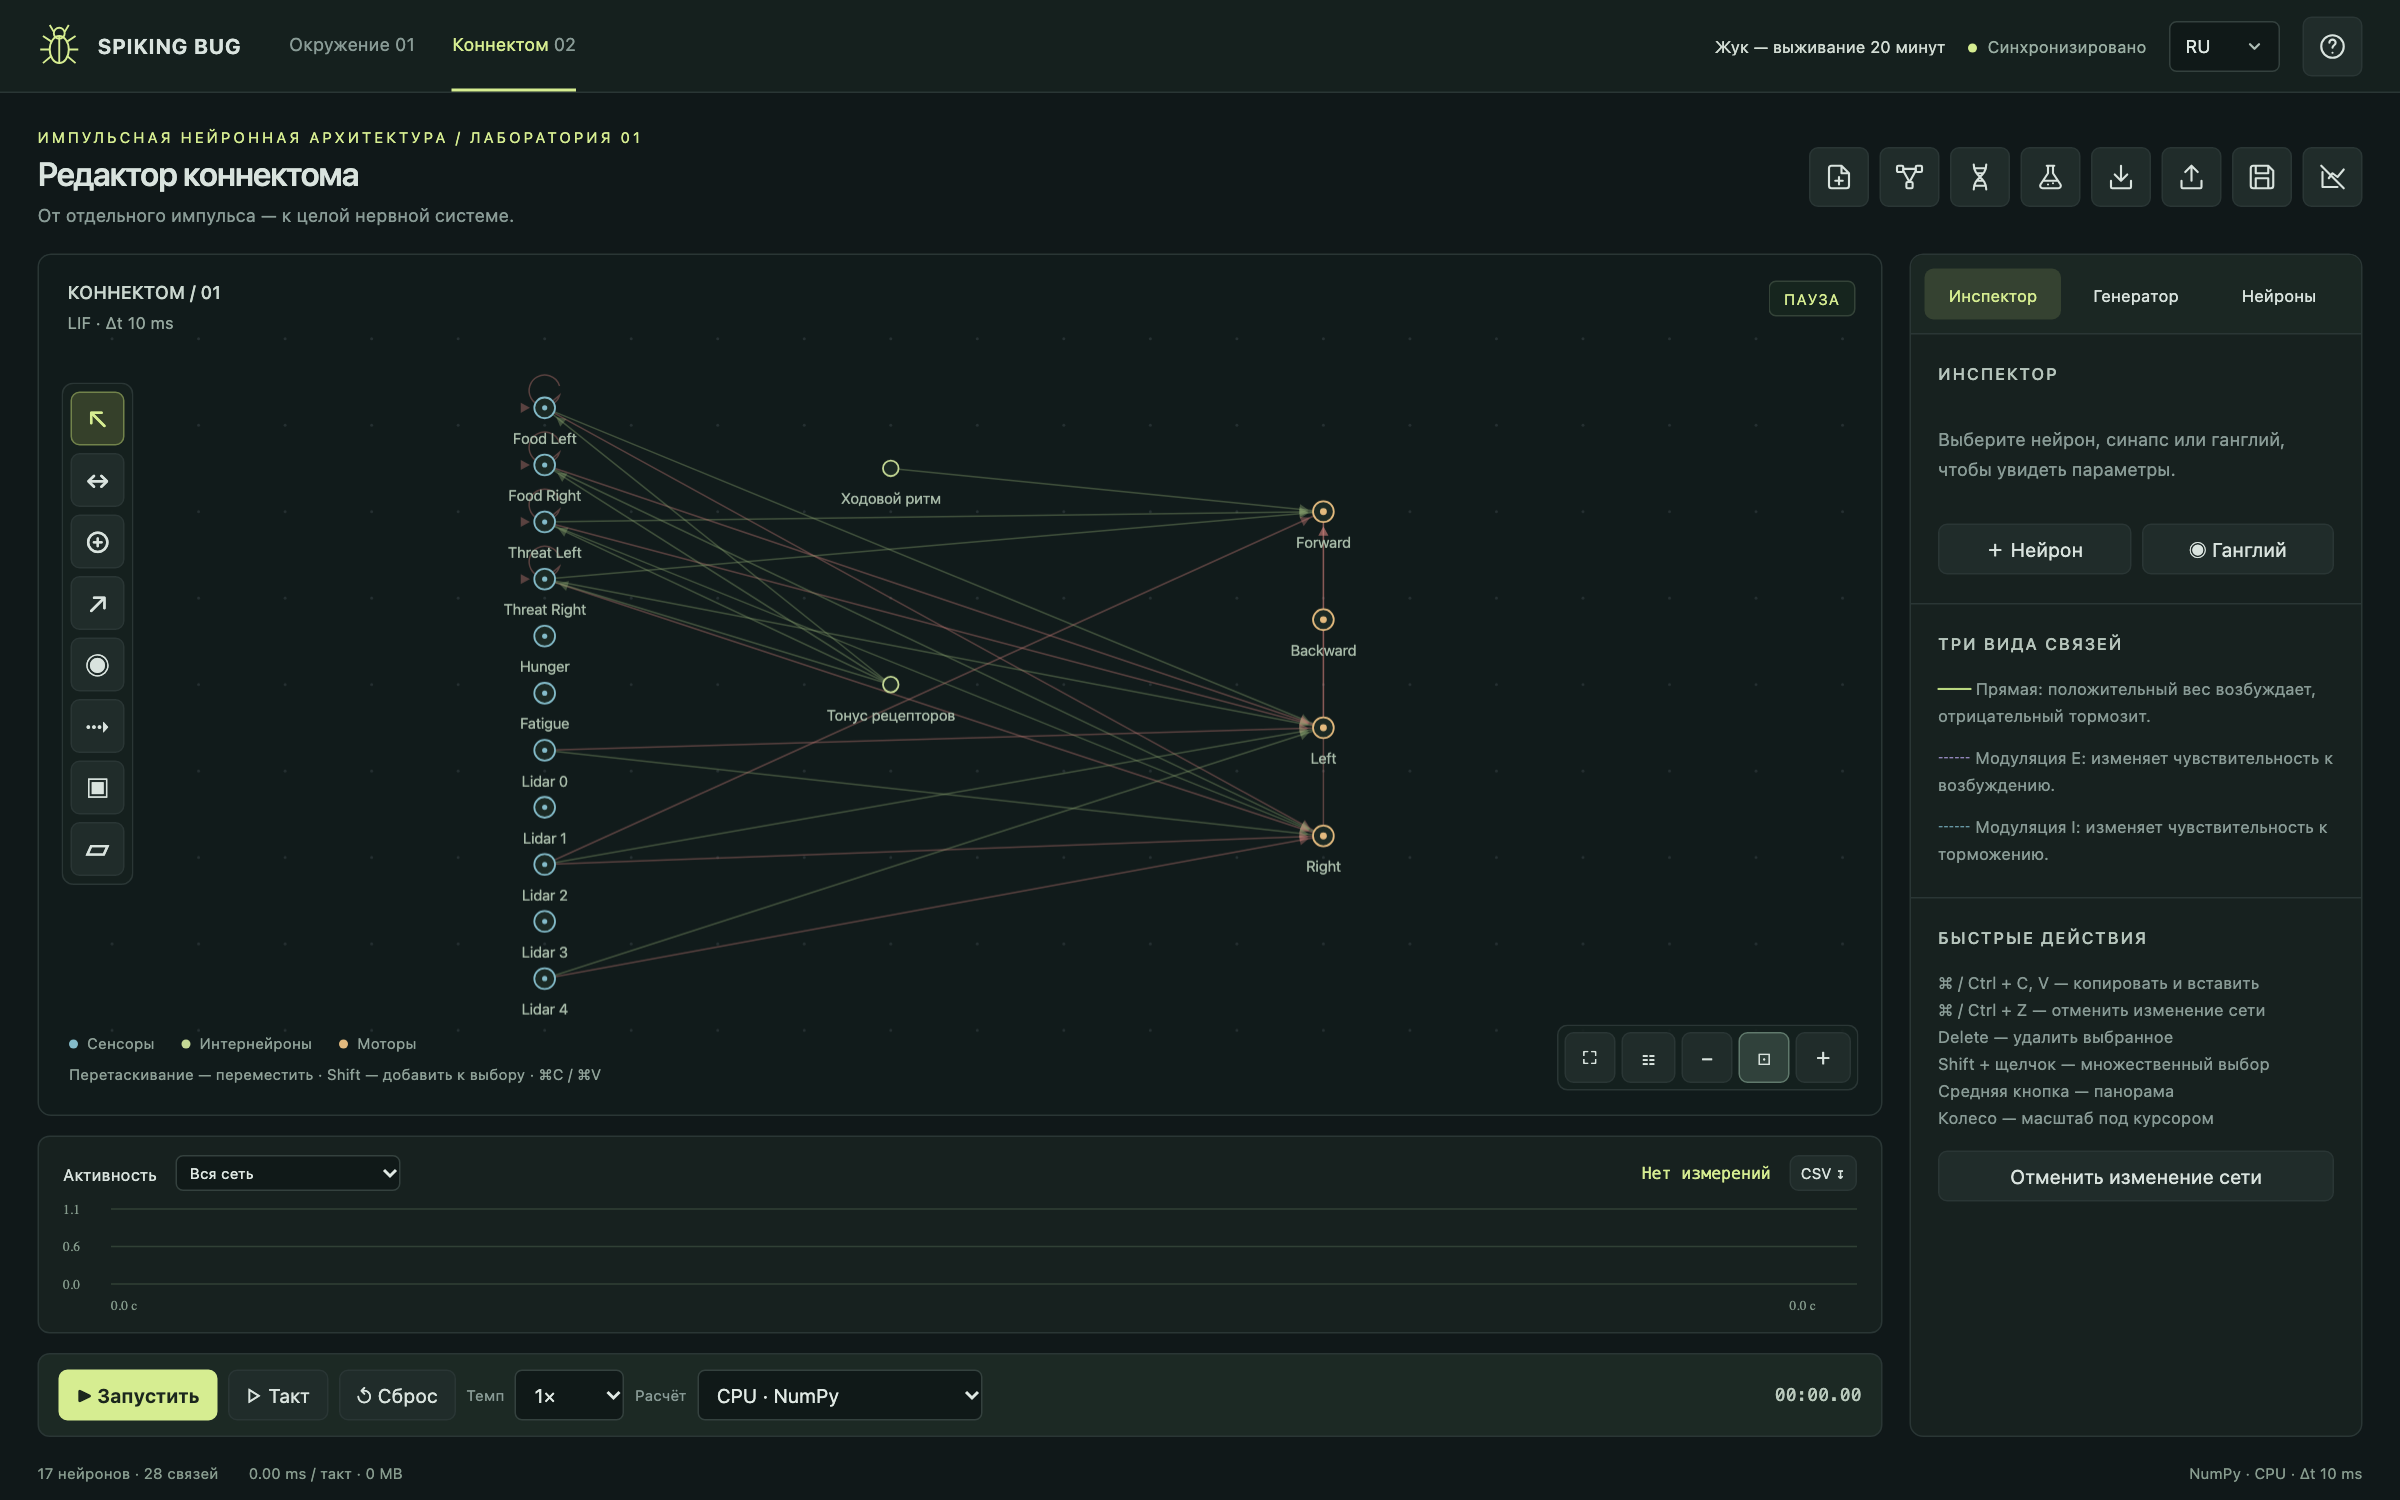
\includegraphics[width=0.98\linewidth]{editor-direct-ru.png}\par\vspace{4mm}
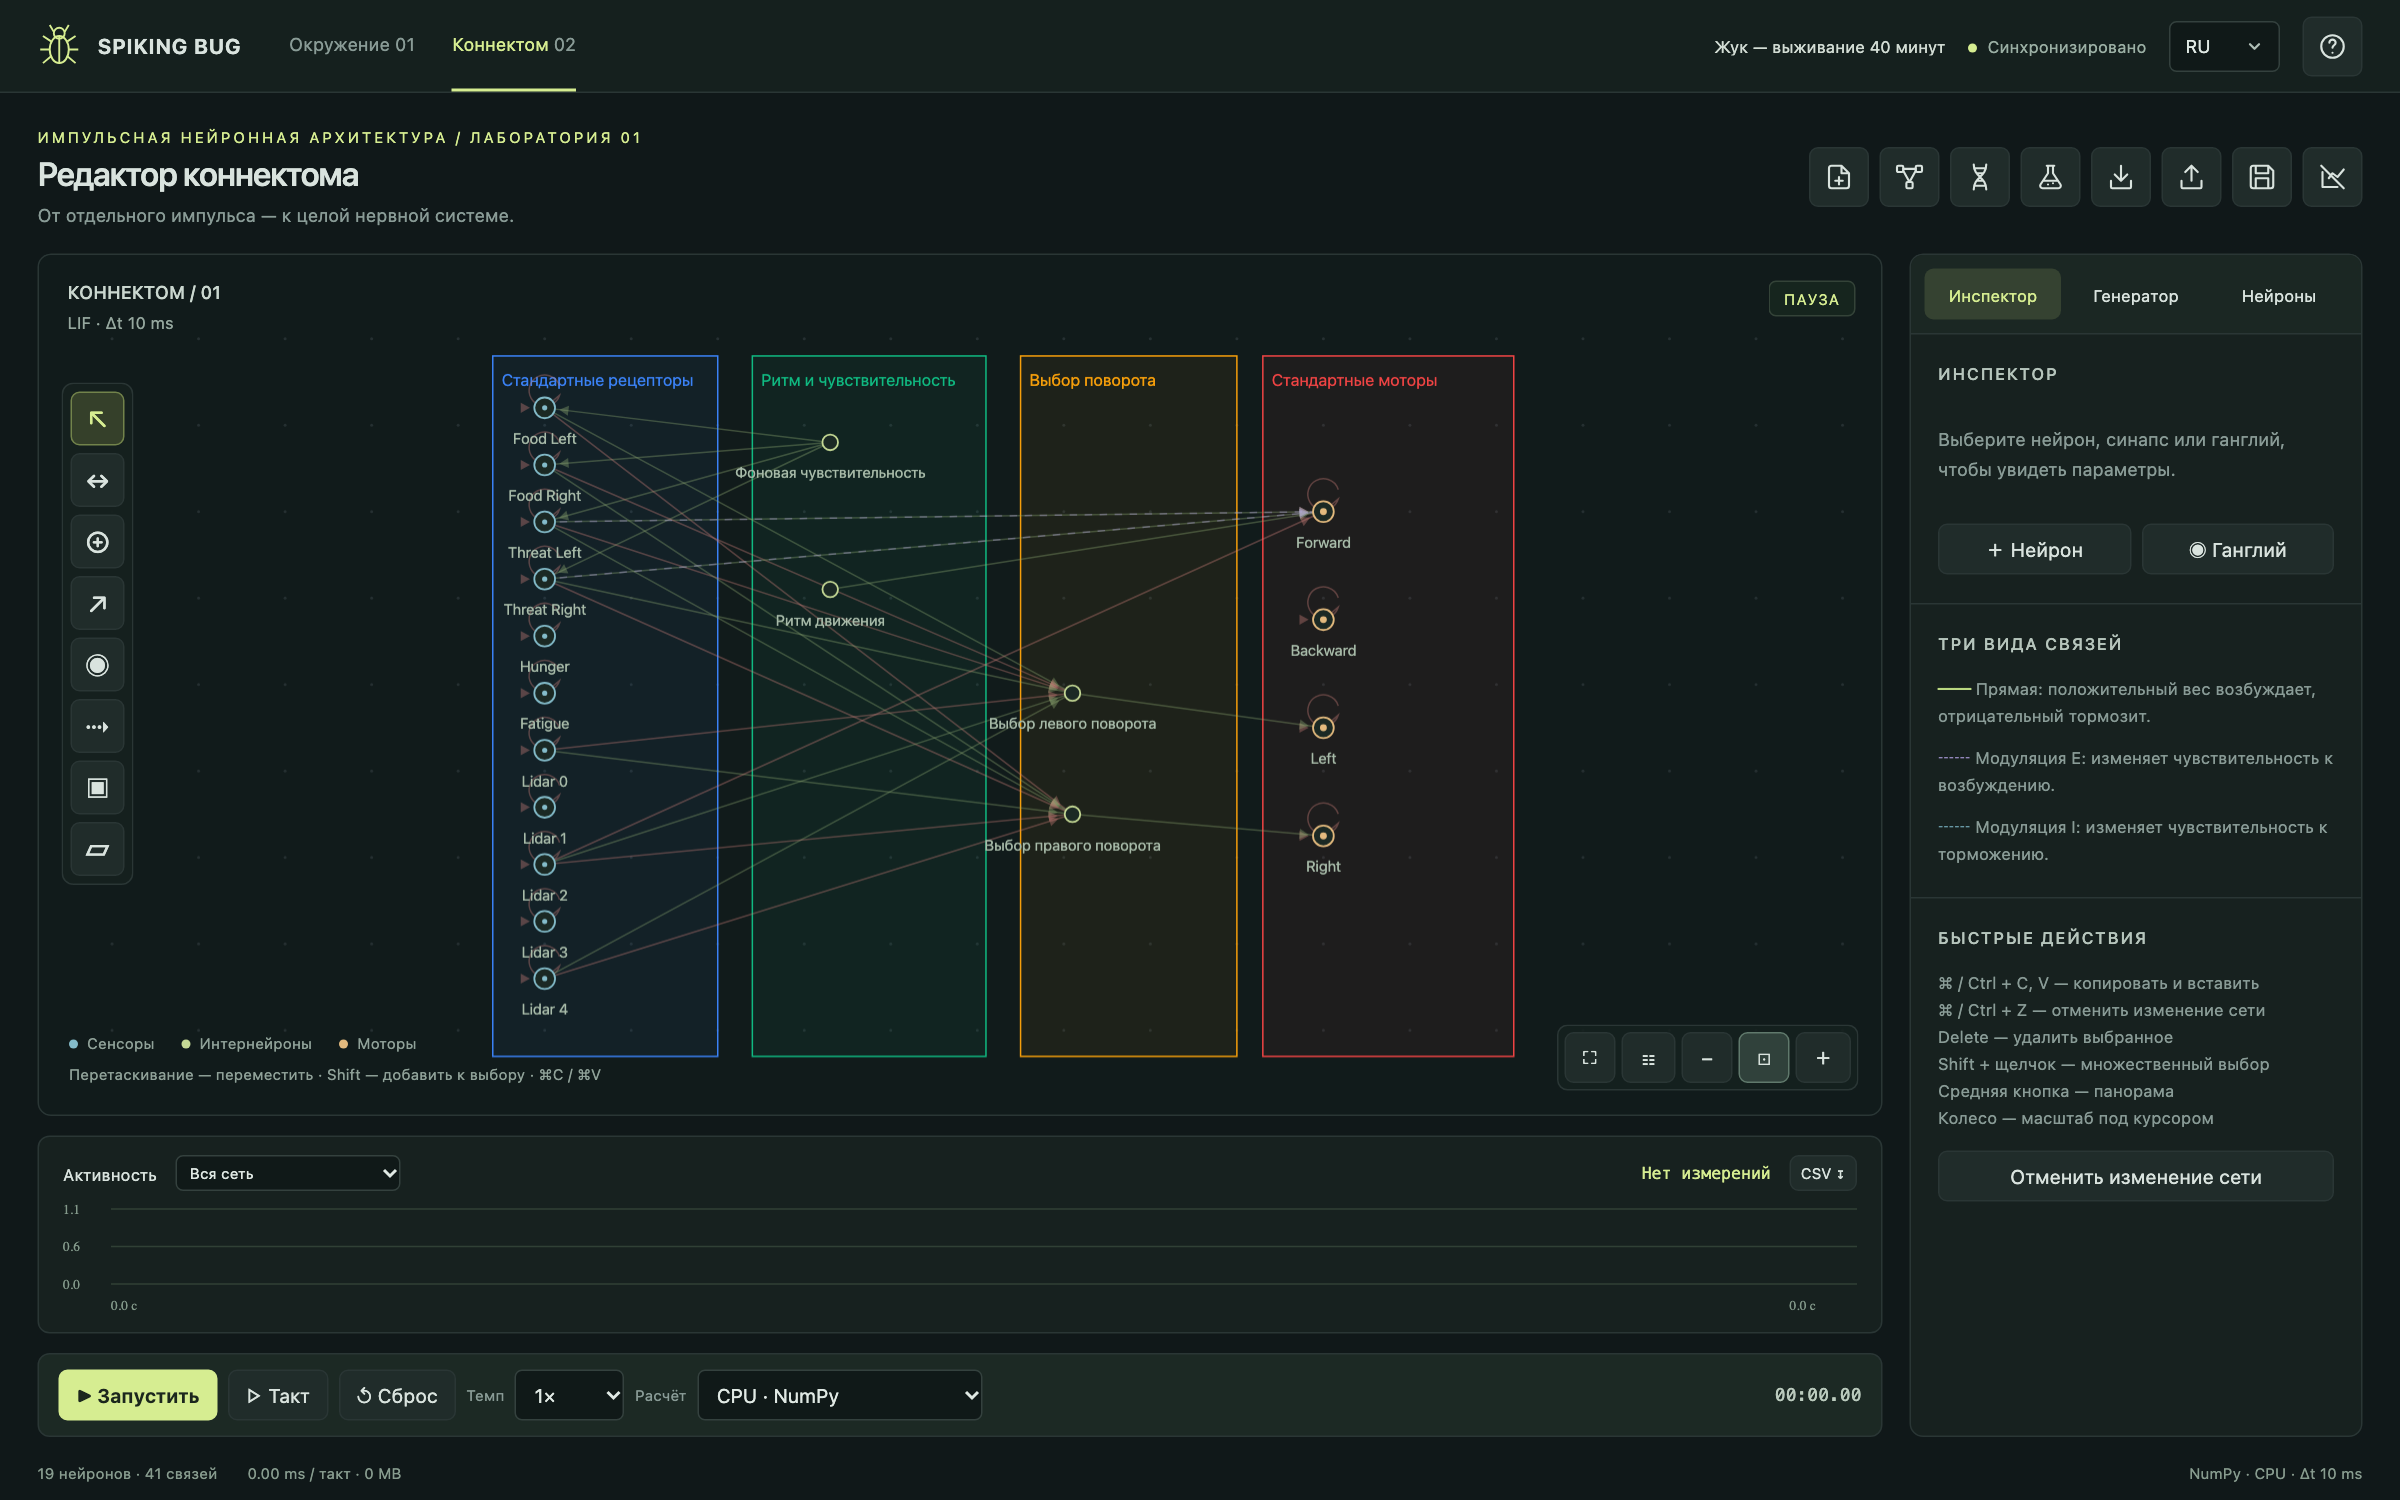
\includegraphics[width=0.98\linewidth]{editor-modulation-ru.png}
\caption{Редактор коннектома со схемами D (сверху) и M (снизу), поставленными на паузу сразу после импорта. Это разные целостные конструкции; M не получена в данном эксперименте простым добавлением двух модулирующих связей к неизменной D.}\label{fig:small}
\end{figure}
\begin{figure}[tbp]\centering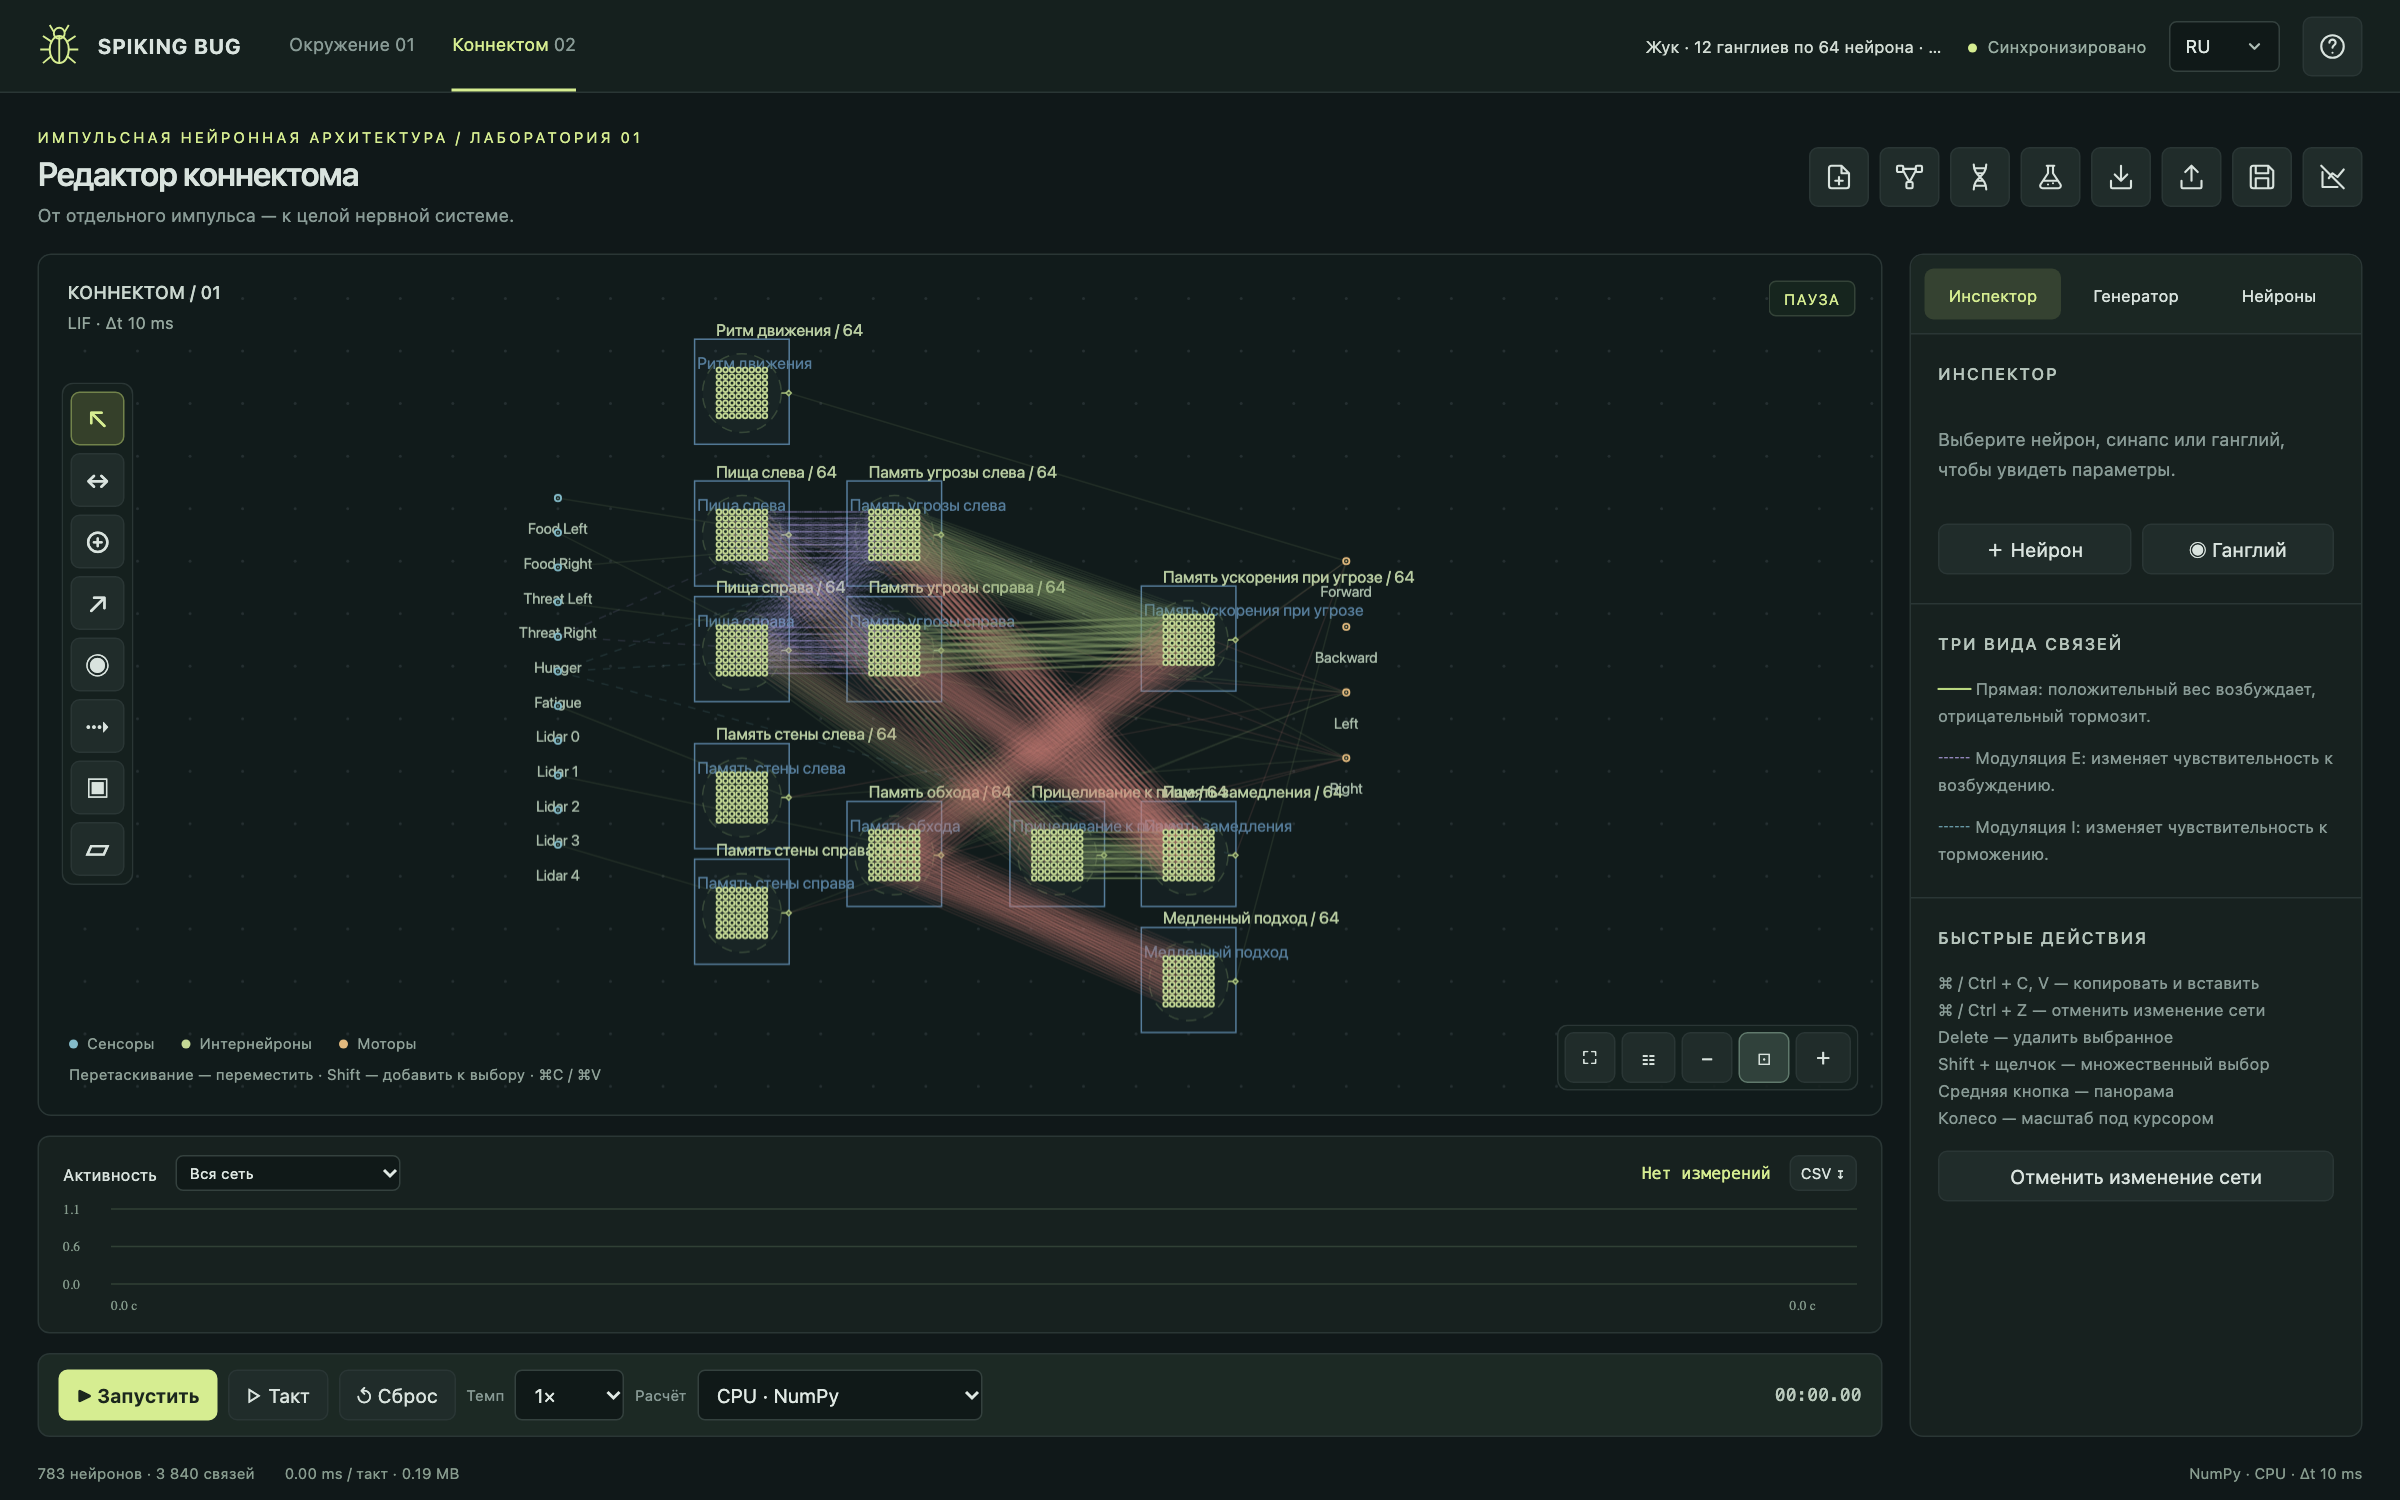
\includegraphics[width=\linewidth]{editor-ganglia-populatio-ru.png}
\caption{Схема G в редакторе: 12 групп по 64 нейрона, периферические сенсорные и моторные нейроны, межпопуляционные проекции. Исходные подписи отражают предполагаемые функции, но не являются независимым доказательством специализации. Плотное расположение подписей сохранено таким, каким оно отображается в существующем редакторе.}\label{fig:ganglia}
\end{figure}

\subsection{Тело агента и среда}
Арена представляет собой ограниченную область $2400\times1600$ с круглым агентом радиуса 12. Одиннадцать каналов кодируют пищу слева/справа, угрозы слева/справа, голод, усталость и пять направлений лидара. Четыре моторных канала задают движение вперёд, назад и поворот влево/вправо. Назначение определяется идентификатором нейрона, а не его подписью или внешним видом. Сенсорные значения ограничены диапазоном $[0,1]$ и прибавляются к входам назначенных нейронов каждый такт. Одновременные моторные команды допускаются.

Моторный спайк преобразуется в движение с длительностью команды 0.04 с внутри шага мира 0.01 с. При номинальной скорости 150 команда вперёд запрашивает перемещение на шесть единиц; для движения назад используется множитель 0.7. Команда поворота задаёт $3\times0.04=0.12$ рад. Поэтому фактическая скорость определяется не только настройкой скорости тела, но и спайковым рисунком, рефрактерностью, сочетаниями команд и столкновениями. Преследователи перемещаются с шагом мира при номинальном отношении скоростей 0.5.

Контакт с пищей сбрасывает голод и восстанавливает до 0.12 здоровья. Голод увеличивается на 0.02 в секунду; при полном голоде здоровье уменьшается на 0.015 в секунду. Контакт с угрозой отнимает 0.25 здоровья в секунду. У угроз радиус обнаружения равен 380, длительность преследования --- пяти секундам, отдых --- четырём, время существования --- 60 с. Целевые количества пищи и угроз равны 35 и трём; пополнение пищи проверяется каждые 0.3 с. В исходных мирах нет внутренних препятствий и зон пищи, поэтому возможности генерации лабиринтов здесь не оцениваются.

Усталость обновляется по правилу
\begin{equation}
 f_{t+1}=\operatorname{clip}_{[0,1]}\left[f_t+\gamma\sum_k a_k^t+\rho N\Delta t-\delta\Delta t\right],
\end{equation}
где $a_k^t$ --- индикаторы моторных команд, $\gamma=0.025$, восстановление $\delta=0.07\,\mathrm{с}^{-1}$, $N$ --- число нейронов, $\rho$ --- коэффициент нейронных затрат. Моторное слагаемое начисляется за событие команды и не умножается на $\Delta t$. Фактическое перемещение или поворот при полной усталости уменьшает здоровье на 0.01 в секунду. При $\rho=0$ среда не назначает прямой цены за число нейронов. Эти коэффициенты являются правилами симулятора, а не калиброванной моделью метаболизма.

\subsection{Протокол, контрольные условия и показатели}
Основное сравнение оценивает D, M и G на seed 21000--21059 с горизонтом $\tau=1200$ с. Сначала была завершена и рассмотрена оценка на том же наборе с горизонтом 600 с. После получения от автора исходной цели «20 минут» горизонт расширили до 1200 с, не меняя схем и не выбирая новые seed. Первичные данные сохранены отдельно. Это явно описанная корректировка исследовательской оценки, а не заранее зарегистрированная подтверждающая проверка на ещё не просмотренных данных. Единственный предварительный замер скорости на seed 9000 и горизонте 120 с исключён из анализа.

В ходе данной оценки контроллеры не дорабатывались. Поскольку seed исходной оптимизации неизвестны, пересечение с прежними испытаниями агента исключить нельзя; набор не объявляется доказанно отложенным относительно конструирования. Начальные позиции пищи и угроз создаются штатной процедурой испытаний с сохранением препятствий, исходной позы и конфигурации. Один seed задаёт одинаковое начальное размещение для всех схем. Позднее случайные последовательности могут расходиться вследствие различий в сборе и пополнении пищи и замене угроз. Поэтому применяется парность по seed, а не требование идентичных полных внешних траекторий.

Каждый эпизод создаёт новую сеть и мир, исполняется без синхронизации с реальным временем и заканчивается при первом обнулении здоровья или достижении горизонта. Интерактивная среда устроена иначе: движение может продолжаться после нулевого здоровья, а пища --- восстановить его. Здесь используется штатная оценка до первой смерти. Единицей повтора является блок seed; такты симуляции не считаются независимыми наблюдениями.

В двух дополнительных условиях из M либо G удаляются все связи \code{mod_exc} и \code{mod_inh}; нейроны, прямые связи и параметры сохраняются. Ещё три условия повторяют D, M и G при $\rho=0.001$ на нейрон в секунду. Всего получается $8\times60=480$ эпизодов на итоговом горизонте. Единственный ненулевой коэффициент --- проверка чувствительности к модельной цене, а не измерение энергопотребления. Дополнительно на seed 21000--21002 сравниваются исходная G и её явный развёрнутый граф. Диагностика M на одном фиксированном seed сравнивает последовательности спайков полной сети и абляции при входах замкнутого контура полной сети. Ещё три описательных испытания используют исходную сохранённую сцену с seed 42 без начальной рандомизации.

Основной показатель выживания --- ограниченное среднее время жизни (restricted mean survival time, RMST):
\begin{equation}
\widehat{\operatorname{RMST}}(\tau)=\frac{1}{n}\sum_{j=1}^n\min(T_j,\tau).
\end{equation}
При цензурировании только общим горизонтом оно равно средней зарегистрированной длительности. Этот показатель не требует экстраполировать ненаблюдаемые времена смерти \citep{royston2013}. Дополнительно учитываются доля выживших к 1200 с, число порций до завершения, пища за минуту жизни, путь, итоговое здоровье, блокировка движения и средняя частота спайков. Счётчик повреждений включает угрозы и истощение, но не потерю здоровья от голода, поэтому не равен полному урону. Скорость сбора пищи нормируется временем жизни и должна рассматриваться вместе с выживанием.

Для непрерывных показателей используются 20\,000 бутстреп-выборок блоков seed и перцентильные 95\%-ные доверительные интервалы (seed генератора 20261021). Парные контрасты строятся по разностям внутри seed. Для долей выживших вычисляются интервалы Уилсона. Интервалы описывают вариативность сцен для фиксированных контроллеров, а не неопределённость класса независимо построенных сетей. Дополнительные контрасты имеют исследовательский характер; интервалы не скорректированы на множественные сравнения, и подтверждающее утверждение о статистической значимости не делается. Эпизоды по результату не исключаются. Используется CPU/NumPy; версии программ и сведения о машине записаны в протоколе.

\section{Результаты}
\subsection{Сопоставление исходных схем}
Таблица~\ref{tab:baseline} и рис.~\ref{fig:performance} показывают выраженную последовательность по сбору пищи: средние D, M и G равны соответственно \DFood{}, \MFood{} и \GFood{} порций за эпизод. Парная разность M--D составляет \MDdiff{} порций (95\% ДИ от \MDlo{} до \MDhi{}), G--M --- \GMdiff{} (от \GMlo{} до \GMhi{}). Это сравнение целостных схем в одном семействе сред.

В отдельной описательной проверке исходной сохранённой сцены на seed 42 все три контроллера доживают до 1200 с, собирая 67, 212 и 399 порций. Эти три эпизода не объединяются со случайной панелью. Таким образом, выполнение первоначальной цели в одной сохранённой сцене совместимо с меньшей устойчивостью при рандомизации.

До горизонта доживают \DSurv{}/60 эпизодов D, \MSurv{}/60 эпизодов M и \GSurv{}/60 эпизодов G. Соответствующие RMST равны \DTime{}, \MTime{} и \GTime{} с. Все эпизоды M и все, кроме одного, эпизоды G достигают горизонта, что создаёт выраженный потолочный эффект. У G наблюдается на одну смерть больше, чем у M; монотонное преимущество по выживанию при увеличении сложности не подтверждается. Ограниченные средние не устанавливают неограниченные времена жизни или устойчивость в более сложных условиях. В частности, преимущество G перед M по пище нельзя автоматически трактовать как доказанное преимущество по продолжительности жизни.

\input{data/baseline-ru}
\begin{figure}[tbp]\centering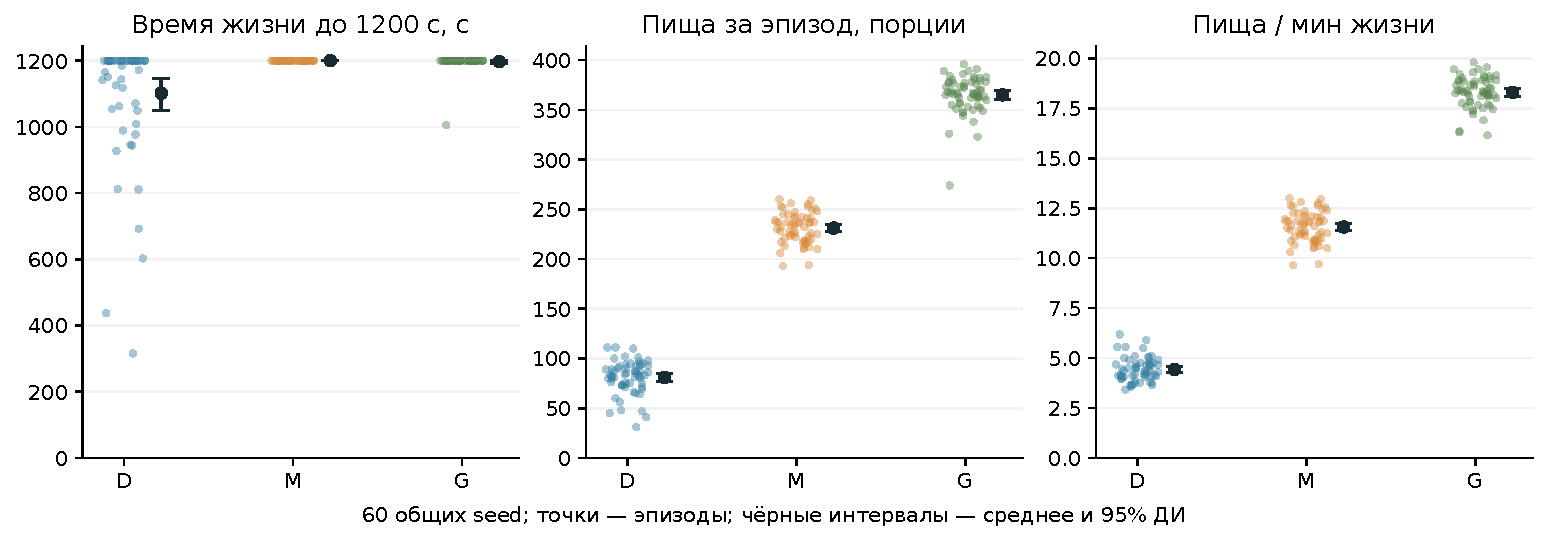
\includegraphics[width=\linewidth]{performance-ru.pdf}
\caption{Показатели исходных схем на 60 общих seed. Цветные точки --- отдельные эпизоды; чёрные точки и интервалы --- средние и бутстреп-ДИ 95\%. Длительность ограничена 1200 с. Скорость сбора пищи нормируется временем жизни.}\label{fig:performance}
\end{figure}

\subsection{Отключение модуляции}
Удаление двух модулирующих возбуждение связей M не изменяет ни одной зарегистрированной длительности, числа порций, скорости сбора, итогового здоровья, повреждений, пути, блокировки или частоты спайков на исследованных seed. Это более конкретный результат, чем отсутствие выявленного различия средних, но он ограничен данным набором входов и показателей. Диагностика на seed 21000 обнаруживает \TraceMismatch{} тактов с различающимися векторами спайков из 120\,000, хотя чувствительность моторного нейрона меняется на \TraceModTicks{} тактах и достигает \TraceMaxSens{}. Моторный нейрон движения вперёд выдаёт 29\,999 спайков за 1200 с (24.999 Гц), практически достигая потолка 25 Гц, заданного тремя рефрактерными тактами и тактом генерации. Эта диагностика поддерживает объяснение через насыщение: дополнительное положительное воздействие не обязано повышать уже максимальную частоту. Следовательно, работающий механизм модуляции может быть избыточным для наблюдаемого поведения.

Для G отключение всей модуляции увеличивает средний сбор с \GFood{} до \GNoModFood{} порций при увеличении числа доживших до горизонта с 59/60 до 60/60. Парная разность «полная схема минус абляция» составляет \GAblDiff{} порций (95\% ДИ от \GAblLo{} до \GAblHi{}). Для данной конструкции и семейства задач модулирующие связи не объясняют преимущество над M; их суммарный вклад в сбор пищи отрицателен. Это не доказывает общего вреда модуляции, а разграничивает наличие механизма и его полезное применение. После абляции схема не перенастраивалась; результат не является оценкой оптимальной сети прямого действия.

\input{data/controls-ru}
\begin{figure}[tbp]\centering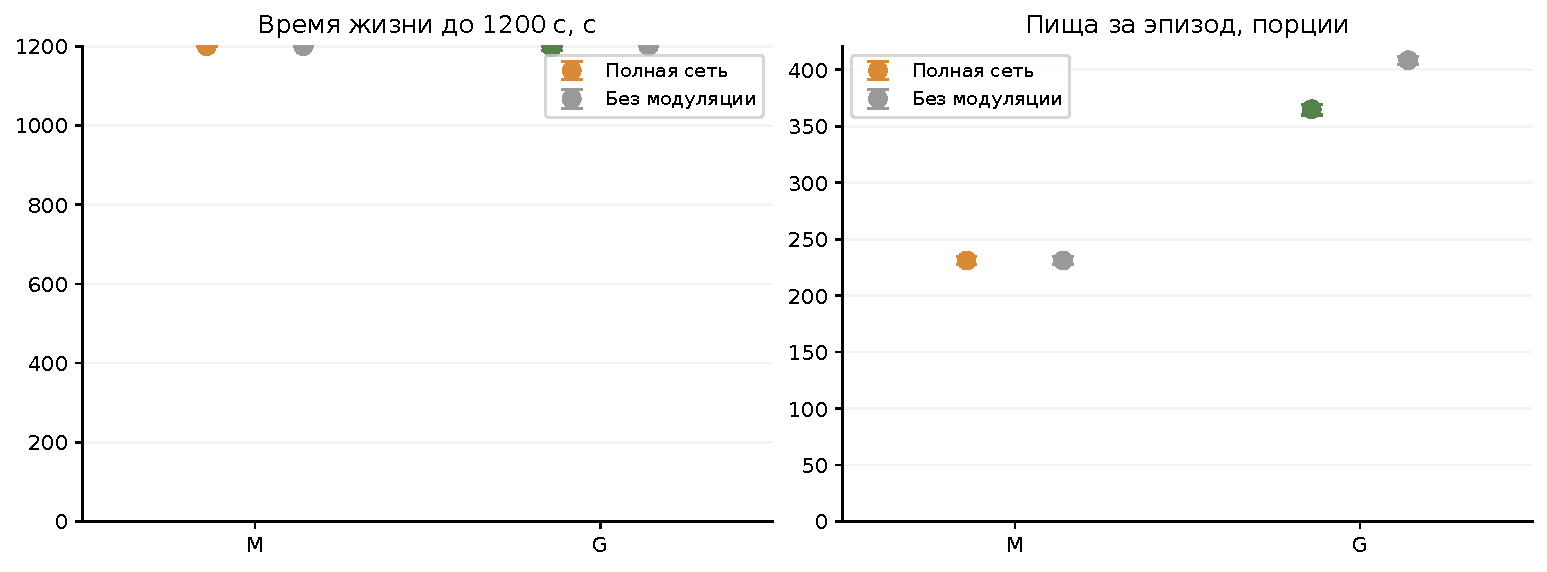
\includegraphics[width=\linewidth]{ablation-ru.pdf}
\caption{Контроль с отключением механизма. Показаны средние и 95\%-ные бутстреп-интервалы полных и лишённых модуляции сетей M и G. Число нейронов и все прямые связи сохранены.}\label{fig:ablation}
\end{figure}

\subsection{Группировка, ресурсы и нейронные затраты}
Развёрнутая G содержит 783 нейрона и 3840 эффективных связей без объектов-ганглиев. Во всех трёх назначенных контрольных повторах её зарегистрированные результаты точно совпадают с исходной сетью. Это соответствует семантике развёртывания: ганглий --- средство конструирования над конкретными нейронами, а не отдельный динамический элемент. Повторы подтверждают эквивалентность реализации на проверенных seed; более общее объяснение заключается в равенстве развёрнутых графов.

G содержит примерно в 46.1 раза больше нейронов, чем D, и в 41.2 раза больше, чем M. Поэтому больший сбор пищи не означает большей ресурсной эффективности. Деление среднего количества пищи на число нейронов даёт \DFoodPerNeuron{}, \MFoodPerNeuron{} и \GFoodPerNeuron{} порций на нейрон за эпизод. Такая нормировка --- описательный показатель, а не измерение энергии или биологического оптимума. Нервная передача имеет различные энергетические составляющие \citep{attwell2001}, которые невозможно адекватно выразить одним числом клеток.

При $\rho=0.001$ добавки усталости до восстановления равны 0.017, 0.019 и 0.783 в секунду. Итоги приведены в табл.~\ref{tab:cost}; модельная цена не отождествляется с энергией. Длительность, сбор пищи, итоговое здоровье и путь совпадают с базовыми значениями для каждого seed всех трёх схем; при этом накопленные повреждения и частоты спайков меняются в части эпизодов. Следовательно, вмешательство действует, но не разделяет основные поведенческие показатели на данном наборе. Ограничение усталости сверху и зависимость урона от движения могут приводить к тому, что большое изменение номинальной цены даёт относительно небольшой поведенческий эффект. Отсутствие сильного ухудшения не доказывает низких метаболических затрат большой сети.

\input{data/cost-ru}
\begin{figure}[tbp]\centering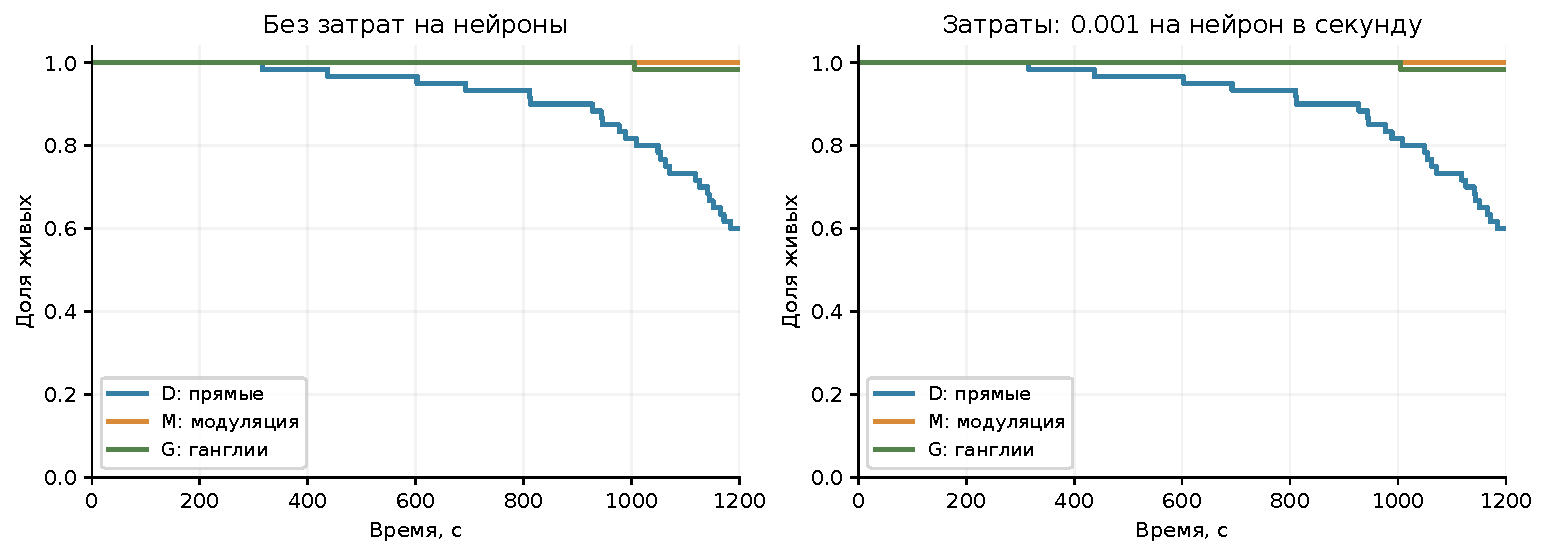
\includegraphics[width=\linewidth]{survival-ru.pdf}
\caption{Эмпирические кривые выживания без цены за число нейронов и в единственном условии с такой ценой. Цензурирование происходит только на общем горизонте. Кривая на единице означает отсутствие смертей до 1200 с, а не неограниченную жизнеспособность.}\label{fig:survival}
\end{figure}
\begin{figure}[tbp]\centering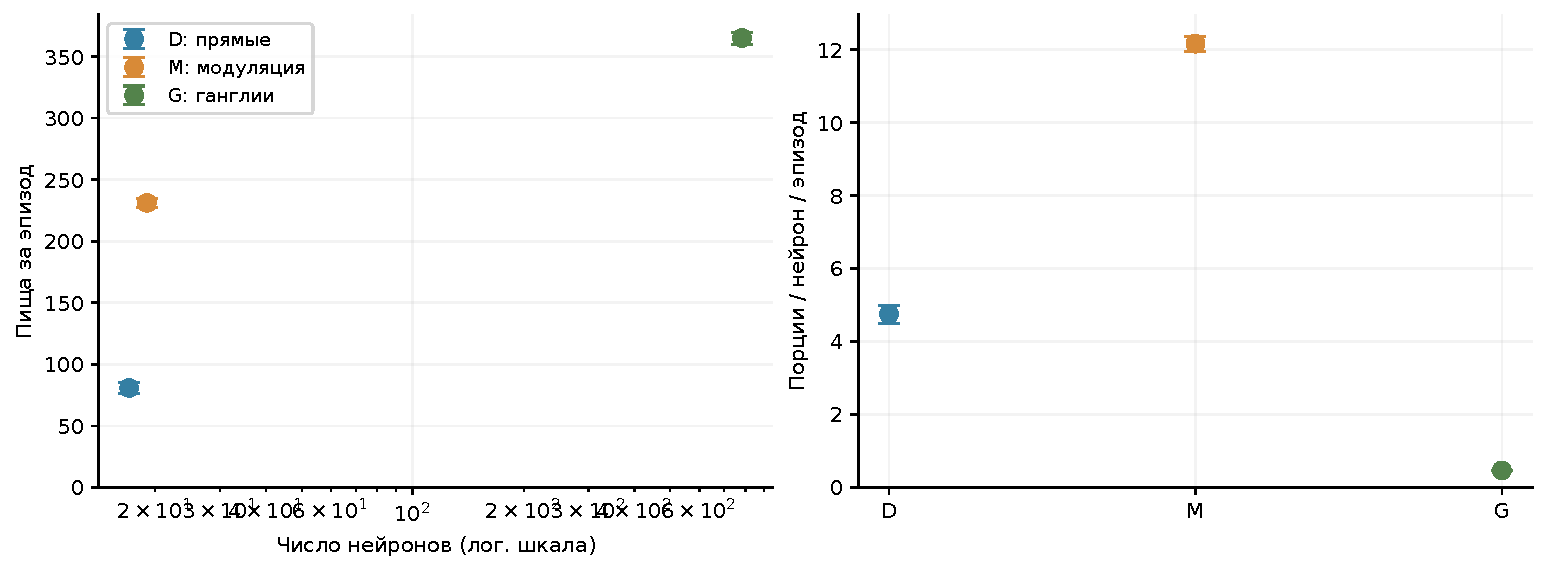
\includegraphics[width=\linewidth]{resources-ru.pdf}
\caption{Сбор пищи в зависимости от числа нейронов (слева) и число порций, делённое на число нейронов (справа), с 95\%-ными бутстреп-интервалами. Число нейронов слева дано в логарифмическом масштабе. Правый показатель не является измерением энергии.}\label{fig:resources}
\end{figure}

\section{Обсуждение}
\subsection{Что показывает последовательность возможностей}
Три схемы иллюстрируют содержательное расширение средств, доступных конструктору. Прямые взаимодействия задают непосредственные положительные и отрицательные воздействия; модуляция добавляет зависимую от контекста динамику усиления; популяции предоставляют способ создавать и соединять повторяющиеся нейронные структуры. Это позволяет ставить более точные вопросы о поведении и представлении. Однако из такой последовательности не следует монотонное улучшение каждой сети по любому показателю.

Порядок по сбору пищи действительно наблюдается у исследованных LLM-созданных схем. Исходное сравнение не устанавливает его причину: одновременно различаются размер, прямые веса, утечка, смещения и топология. Абляции существенно сужают интерпретацию: преимущество M перед D сохраняется без модуляции, а сбор G после её удаления увеличивается. Поэтому выдавать основной график за доказательство улучшения именно вследствие появления модулирующих синапсов было бы некорректно.

Отрицательный механистический результат делает исследование методологически содержательнее. Среда может корректно реализовывать биологически мотивированную возможность, которую конкретный пример не использует с пользой. Представление может облегчать создание сложных схем, хотя сама группировка не меняет поведение развёрнутого графа. Проверка промежуточных механизмов позволяет избежать превращения привлекательного эволюционного объяснения в неподтверждённую причинную историю.

\subsection{От возможностей к эволюционируемости}
Эволюционные алгоритмы способны изменять архитектуру и параметры согласно критерию отбора \citep{floreano2008}. В Spiking Bug имеется отдельная подсистема мутаций и отбора, но для представленных результатов эволюционный поиск не запускался. Поэтому не заявляются преимущества по поколениям, скорости поиска, адаптации или появлению новизны. Наличие такой подсистемы в коде не превращает сравнение фиксированных схем в эволюционный эксперимент. Итеративное конструирование агентом LLM также представляет другой процесс поиска.

Прямая проверка эволюционируемости потребует независимых запусков поиска для каждого представления, фиксированных обучающих и валидационных сцен и заключительного неизменяемого тестового набора. Размер популяции, бюджет оценок, лимиты нейронов/связей и доступные мутации следует согласовать или изучать как отдельные факторы. Нужны несколько seed самого поиска: 60 сред для одного контроллера не заменяют 60 независимых линий. Групповые мутации или дупликации можно сопоставить с мутациями явного графа при одинаковом бюджете после развёртывания. Тогда гипотеза приобретёт измеримую форму: повышают ли новые правила построения вероятность или скорость достижения заданного уровня на отложенных сценах?

Для проверки именно LLM-конструирования нужен сходный, но отдельный дизайн: независимые сессии агента на каждое условие, фиксированный системный контекст, одинаковое число обращений к модели и испытаний, сохранённые кандидаты и единый критерий завершения. Общий промпт полезен, но сам по себе не обеспечивает эти условия. Данные настоящей работы относятся к полученным трём артефактам, а не к распределению успеха GPT-6 Astra.

\subsection{Зависимость от задачи и биологическая интерпретация}
Открытая арена предъявляет требования к устойчивому сбору ресурсов при ограниченном сенсорном интерфейсе. Она не проверяет отложенное вознаграждение, смену контекста, многоэтапные решения, обобщение на лабиринты и перенос между экологиями. Такие задачи могут сильнее выявлять пользу затухающего модуляторного состояния или повторно используемых популяций. Однако их следует выбирать до анализа выгодных исходов; иначе постфактум можно создать кажущееся преимущество механизма.

Биологически оправданная аналогия состоит в расширении и реорганизации доступных способов управления при экологических ограничениях. Полученные результаты не устанавливают порядок появления нейромедиаторов, ганглиев или централизации. Они также не предполагают универсального наращивания сложности: компактный контроллер может быть экономичнее в конкретной задаче. Исследования диффузной химической сигнализации и конвергентной организации нервных систем согласуются с разнообразием траекторий, а не с единственным направлением от простого к сложному \citep{jekely2021,martin2018}.

\subsection{Ограничения}
Главное ограничение --- по одному контроллеру на категорию. Все интервалы условны относительно этих файлов. Общий промпт контролирует инструкции, но не гарантирует беспристрастность: модель может иметь архитектурные предпочтения, а разные запуски --- получать разный объём обратной связи из испытаний. Проверяется устойчивость к рандомизации сцены, а не эффект класса архитектур в популяции независимо построенных решений.

Неизвестны число исходных итераций LLM, seed испытаний, история отбора и затраты вычислений. Отсутствие ограничений размера соответствует полученному промпту, но не уравнивает ёмкость схем. Большая разница размеров смешивает влияние механизмов и числа элементов; отдельно оптимизированная прямая сеть сопоставимого размера не исследована.

Отсутствие внутренних препятствий ограничивает выводы о навигации, а конечный горизонт --- о выживании. Один коэффициент затрат не определяет границу компромисса между эффективностью и энергией. Нулевой нейронный шум оставляет случайность только в среде. Проверено исполнение на CPU; численное соответствие GPU и аппаратное энергопотребление не измерялись. Наконец, упрощённые нейроны, скалярная чувствительность и плоское тело являются функциональными абстракциями: конкретный биологический вид или анатомический коннектом не реконструируются.

\section{Заключение}
Spiking Bug объединяет в исполнимой среде прямую передачу, модуляцию чувствительности и популяционное построение нервных схем. Три подготовленных контроллера показывают последовательное увеличение сбора пищи при парной оценке на 60 сценах. Выживание различает простую и более сложные схемы, однако переход M--G не даёт монотонного улучшения, а горизонт 1200 с создаёт существенное цензурирование. Контрольные условия показывают, что модуляция не требуется для наблюдаемого поведения M и уменьшает сбор пищи у исходной G, а развёртывание ганглиев сохраняет поведение. Обоснованный вывод состоит в том, что более богатые средства проектирования позволяют создавать сложные эффективные конструкции, однако вклад каждого механизма и преимущество по каждому критерию должны быть проверены отдельно. Их роль в повышении эволюционируемости остаётся явной воспроизводимой исследовательской гипотезой.

\section*{Доступность материалов и статус рукописи}
В комплект входят три исходных JSON-файла и их хеши; протокол; 480 итоговых эпизодов в JSONL и CSV; отдельные данные первоначального 600-секундного опыта; сводная статистика; проверки развёртывания и спайковых последовательностей; векторные графики; исходные скриншоты; скрипты расчёта и съёмки; снимок Python-кода среды; обе версии LaTeX и PDF. Публичный архивный DOI и предоставление лицензии не заявляются. Это исследовательская рукопись для проверки автором, а не рецензированная публикация. Перед подачей автору необходимо указать или подтвердить аффилиацию, ORCID, финансирование, конфликт интересов и журнал; эти сведения не выводятся из email. При анализе кода, выполнении экспериментов, поиске литературы, подготовке текста, переводе и иллюстрациях использовалась помощь ИИ; автору следует проверить материалы и согласовать формулировку раскрытия с правилами журнала.

\FloatBarrier
\appendix
\section{Промпт конструирования и происхождение данных}
Автор предоставил следующий исходный промпт для варианта прямого действия. Неформальные формулировки сохранены. Это предоставленное автором свидетельство о постановке задачи, а не извлечённый журнал работы модели.
\begin{quote}\small
так у тебя задача\\
собрать нервную схему для жука так чтобы он проходил испытание и выживал на 20 минут\\
тебе можно только создавать файл сохранения, код и настройки менять нельзя\\
можно использовать только побудительные и тормозящие синапсы, нет ограничения в количестве нейронов и синапсов\\
начинаешь с пустой нервной системы где есть только дефолтные рецепторные и моторные нейроны\\
можешь делать итерации создание схемы - проверка испытанием - оценка того как можно улучшить - доработка схемы и так по циклу пока не получишь приемлемый результат.
\end{quote}
Редакционная формулировка: «Создайте нервную схему жука, обеспечивающую выживание в 20-минутном испытании. Разрешено создавать только файл сохранения; изменять код и настройки среды нельзя. Используйте только возбуждающие и тормозящие синапсы, без ограничения числа нейронов и связей. Начните с дефолтных рецепторных и моторных нейронов. Повторяйте создание схемы, испытание, анализ и доработку до приемлемого результата». Эта редакция не заменяет исторический текст. В других вариантах, по сообщению автора, менялись допустимые механизмы; точные полные тексты этих промптов отсутствуют.

При повторении исследования следует сохранять все промпты, идентификатор версии модели, журналы инструментов, файлы кандидатов и каждый seed испытания с результатом. Для оценки влияния набора разрешённых механизмов на успех LLM-конструирования нужны независимые повторные запуски. Русский и английский тексты приложения описывают одну постановку; перевод не является отдельным использованным промптом.

\section{Воспроизведение и аудит}
Основной расчёт использует \code{server.trials.run_attempt} и не изменяет активный интерактивный документ. Четыре рабочих процесса независимо вычисляют эпизоды и возвращают результаты в фиксированном порядке. Контрольные условия создаются на копиях документов; исходные файлы неизменны. В \code{runtime_snapshot/server} сохранён использованный код. В ходе оценки не проводятся оптимизация весов, повторное обучение или отбор удобных seed.

В среде Python с зафиксированными зависимостями NumPy и Matplotlib следует выполнить \code{python scripts/experiment.py --workers 4 --horizon 1200}, затем \code{python scripts/analyze.py}; подробные пути для проекта и отдельного архива указаны в инструкции воспроизведения. Повторный расчёт заменяет генерируемые данные, поэтому для сравнения нового запуска следует сохранить поставленный архив. Первые три базовых эпизода G повторяются для проверки развёртывания. Предварительный замер, дополнительные повторы и спайковая диагностика не объединяются с 480 основными эпизодами.

Генератор выполняет 35 начальных размещений пищи и три попытки размещения угроз. Слишком близкие к агенту угрозы могут быть пропущены штатной процедурой; следующие такты пополняют целевое количество. Поэтому одинаковая начальная сцена означает одинаковые правила симулятора для seed, а не искусственно фиксированное число угроз в обход этих правил. Нейронный гауссов шум отсутствует. Скриншоты намеренно показывают сохранённую сцену с seed 42, а все количественные графики строятся по отдельной случайной панели.

Численным источником таблиц и макросов служит \code{data/summary.json}. Каждый доверительный интервал вычисляется по результатам отдельных seed. Полные траектории всех эпизодов не сохранялись: комплект содержит агрегированные записи испытаний и дополнительную диагностику равенства спайков, поэтому не позволяет ретроспективно утверждать свойства незаписанных промежуточных состояний.

\bibliographystyle{plainnat}
\bibliography{references}
\end{document}
